\vspace*{-6mm}
%pre-001
\begin{prerequis}[Connaisances \emoji{red-heart} et compétences \emoji{diamond-suit} du cycle 3]    
   \begin{itemize}        
       \item[\emoji{red-heart}] Vocabulaire associé à ces objets et à leurs propriétés : côté, sommet, angle, hauteur.
       \columnbreak
       \item[\emoji{diamond-suit}] Reconnaître, nommer, décrire des triangles, dont les triangles particuliers (triangle rectangle, triangle isocèle, triangle équilatéral).       
   \end{itemize}
\end{prerequis}
\vspace*{-3mm}
%pre-002
\begin{prerequis}[Connaisances \emoji{red-heart} et compétences \emoji{diamond-suit} du cycle 4]    
    \begin{itemize}        
        \item[\emoji{diamond-suit}] Mener des calculs impliquant des grandeurs mesurables, exprimer les résultats dans des les unités adaptées.
        \item[\emoji{diamond-suit}] Exprimer et vérifier la cohérence des résultats du point de vue des unités.
    \end{itemize}
\end{prerequis}
\begin{debat}[Les mandalas]
    \vspace*{-8mm}
    {\bf Mandala} est un terme sanskrit qui signifie {\it cercle}. Il désigne plus largement un objet support à la méditation et à la concentration composé de cercles; de symétries et de formes diverses. \\
    \vspace*{-3mm}
    \begin{center}
      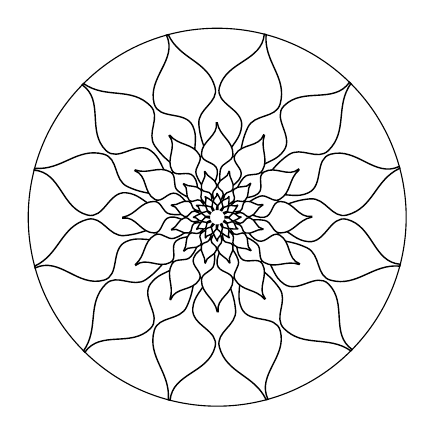
\begin{tikzpicture}[scale=0.2,pics/leaf/.style={code={\pgfgettransformentries{\myxx}{\myxy}{\myyx}{\myyy}{\tmp}{\tmp}\pgfmathsetmacro{\myscale}{sqrt(\myxx*\myyy-\myxy*\myyx)} \draw[line width=0.5,pic actions] (-0.02,0) to[out=80,in=-80] (0,0.1) to[out=100,in=-90] (-0.1,0.2) to[out=90,in=-80] (-0.006,0.4) -- (0,0.4) to[out=-80,in=90] (0.1,0.2) to[out=-90,in=80] (0.02,0.1) to[out=-100,in=95] (0.02,0) -- cycle;}}]
         \path foreach \Radius [count=\Cnt] in {4,2,1,0.5} {foreach \Angle [evaluate=\Angle as \EffAngle using {\Angle-15*\Cnt}] in {0,30,...,330} { (\EffAngle:\Radius) pic[rotate=\EffAngle-90,scale=\Radius,fill=white]{leaf}}};
         \draw (0,0) circle (12) ;
       \end{tikzpicture}
    \end{center}
    \begin{cadre}[B2][J4]
       \begin{center}
          \hrefVideo{https://www.yout-ube.com/watch?time_continue=262&v=bgoHUH-_yWo&feature=emb_logo}{\bf Tibet sand painting of Mandala}, chaîne YouTube {\it Tibet travel}
       \end{center}
    \end{cadre}
 \end{debat}